% Both comparisons reuse paper_q2_results/topic_assignments.csv unchanged.
\subsubsection{Q1-Referenced Trajectory Comparisons}
\label{sec:q1_q2_comparisons}
We evaluated both subtraction options using exactly the same saved rerun assignments, with \emph{no additional topic-model fit}. The Q1 baseline contains 478 tickets and the Q2 target contains 403 tickets. Option~1 has 91 comparable Q2 endpoints. Option~2 has 77 comparable ordinal-day pairs (days 14--90): 13 target days are excluded because the corresponding Q1 startup windows are partial, and Q2 day 91 has no Q1 endpoint. All denominators include noise. Differences are reported in percentage points (pp), not relative percent changes.

\begin{figure*}[t]
    \centering
    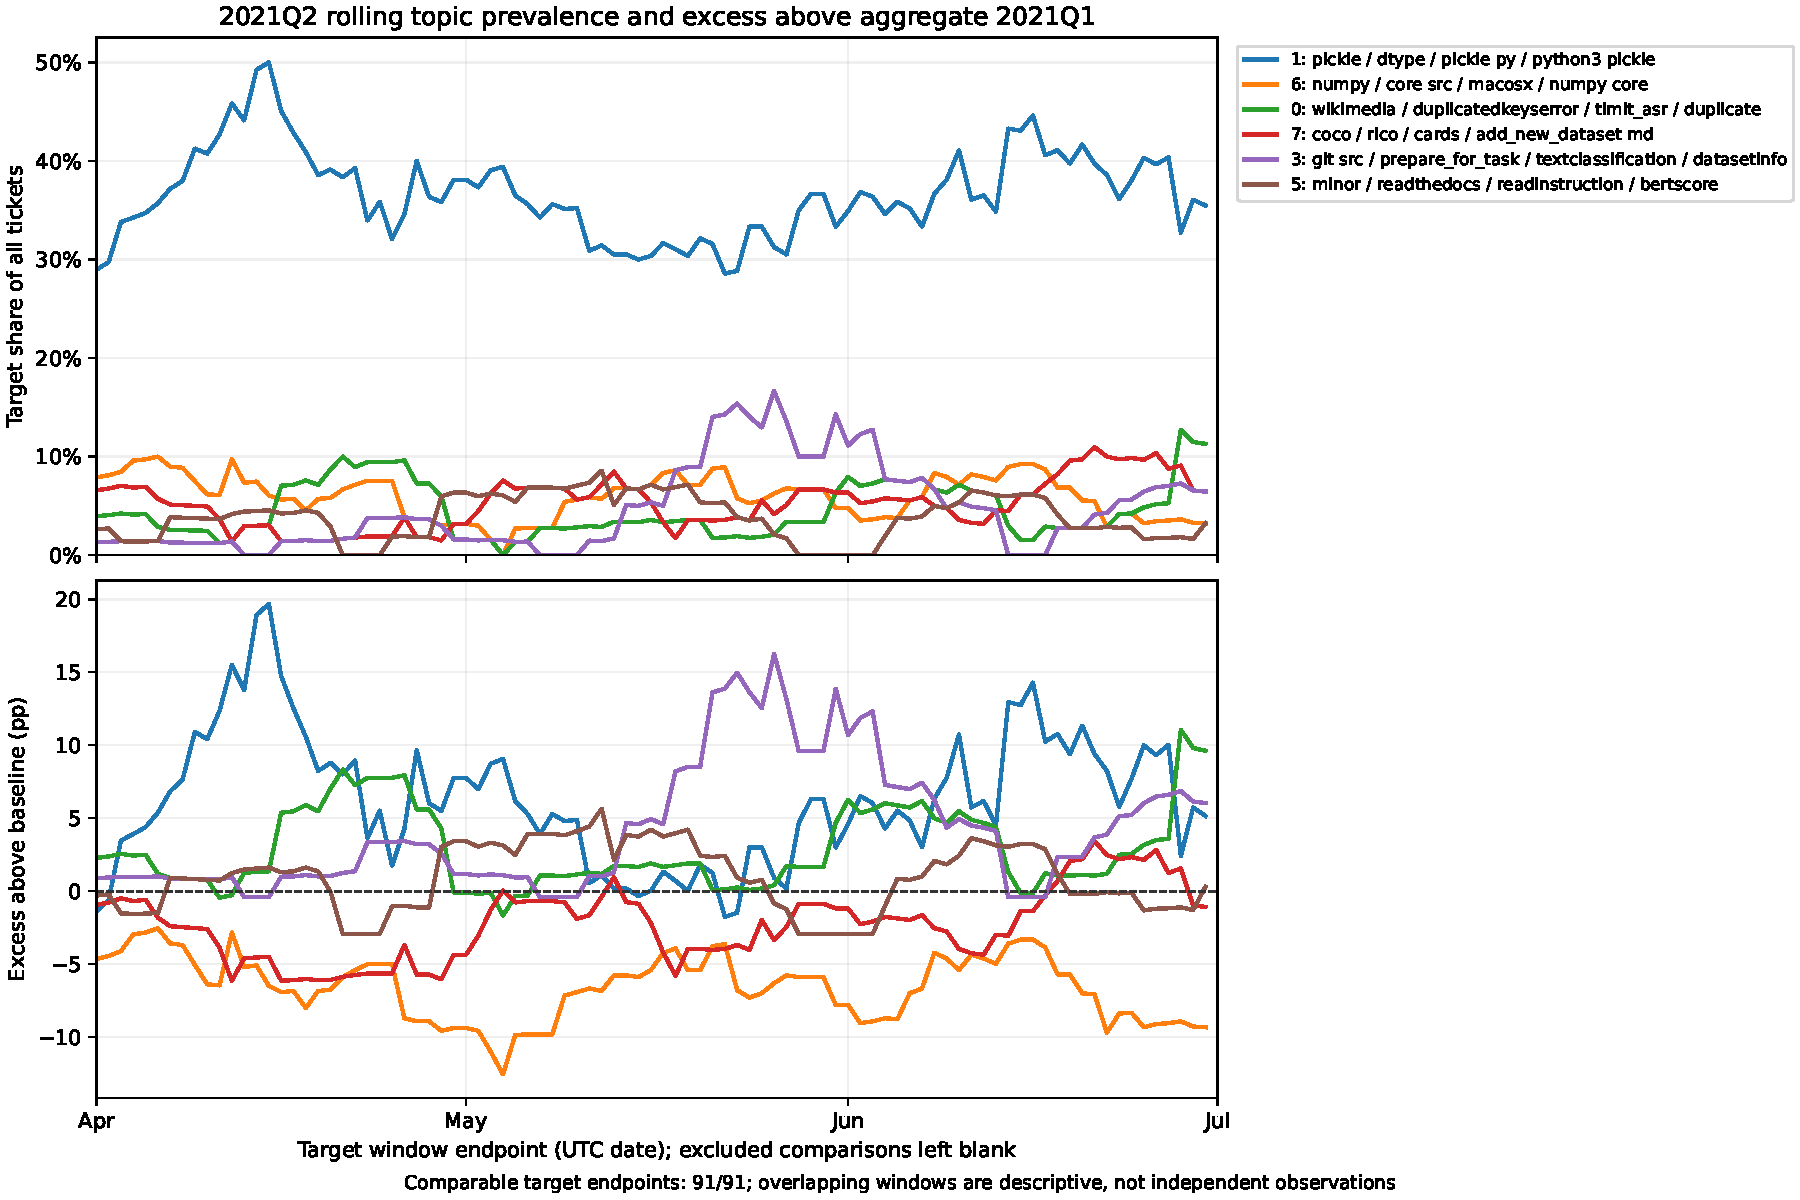
\includegraphics[width=0.98\textwidth]{paper_q2_results/comparisons/baseline_excess_2021Q2_vs_2021Q1.pdf}
    \caption{Option~1: actual Q2 rolling prevalence (top) and excess above the overall Q1 prevalence of the same topic (bottom). The baseline uses original Q1 counts, not the mean of overlapping Q1 windows. Positive values indicate an elevated share relative to Q1; the dashed zero line marks baseline parity. The six non-noise topics are selected by Q2 counts; all denominators retain noise. IDs belong only to the documented same-data rerun.}
    \label{fig:q1_baseline_excess}
\end{figure*}

\begin{figure*}[t]
    \centering
    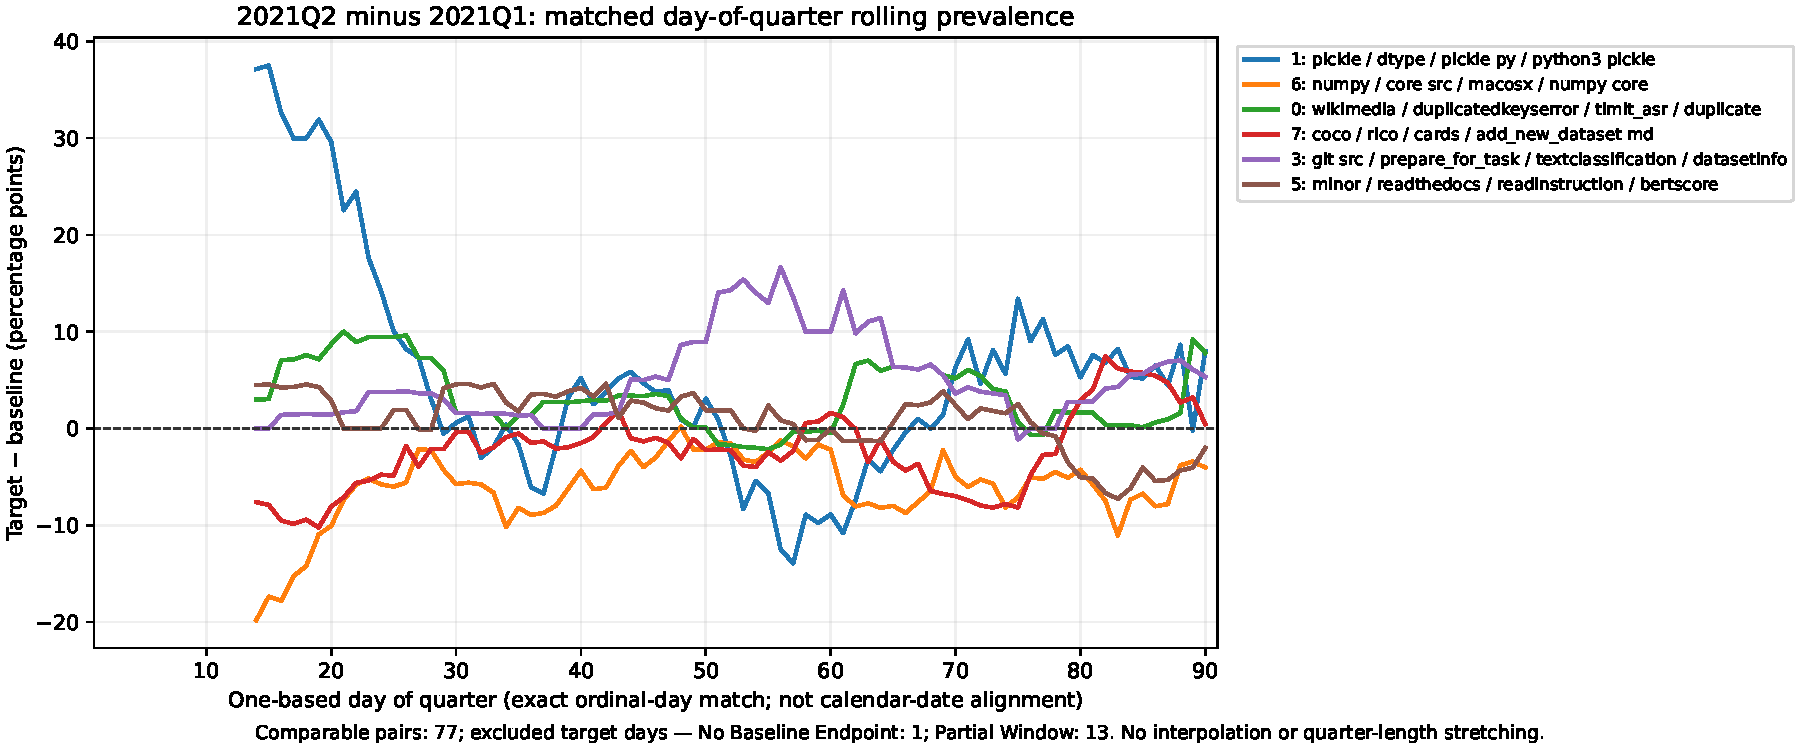
\includegraphics[width=0.98\textwidth]{paper_q2_results/comparisons/aligned_difference_2021Q2_vs_2021Q1.pdf}
    \caption{Option~2: Q2 rolling prevalence minus Q1 rolling prevalence at the same one-based day of quarter. Both windows must be full-length and supported. The 90/91-day timelines are not stretched or interpolated; Q1 startup days 1--13 and unmatched Q2 day 91 have no difference estimate. Ordinal-day alignment is exploratory and does not control for weekdays, holidays, or release events.}
    \label{fig:q1_q2_aligned_difference}
\end{figure*}

\begin{table}[t]
\centering
\small
\begin{tabular}{lrrr}
\toprule
\textbf{Rerun cue} & \textbf{Q1 share} & \textbf{Mean $E$} & \textbf{Mean $D$} \\
\midrule
R1: pickle / dtype & 30.33\% & +6.29 & +5.27 \\
R0: duplicate keys & 1.67\% & +2.92 & +3.34 \\
R3: task casting & 0.42\% & +4.26 & +4.98 \\
R6: numpy / core & 12.55\% & $-6.56$ & $-6.14$ \\
\bottomrule
\end{tabular}
\caption{Descriptive mean differences in pp: $E$ averages 91 Q2 endpoints relative to the overall Q1 baseline; $D$ averages 77 exact ordinal-day pairs. These are different reference constructions and endpoint sets, not independent estimates of the same quantity. R-prefix IDs identify the saved rerun.}
\label{tab:q1_q2_comparisons}
\end{table}

\textbf{Elevation relative to Q1.} Figure~\ref{fig:q1_baseline_excess} shows that the task-casting topic (R3) exceeds its Q1 baseline of 0.42\% at 80 of 91 Q2 endpoints. Its maximum excess is +16.25 pp on May 26, and its mean excess is +4.26 pp. The NumPy/core topic (R6), by contrast, remains below its 12.55\% Q1 baseline at \emph{every} Q2 endpoint, with mean excess $-6.56$ pp. Thus a nonzero absolute Q2 trajectory need not indicate a new elevation over the earlier baseline. These findings describe shifts in share; they do not by themselves establish causes or remediation.

\textbf{Timing relative to the earlier curve.} Figure~\ref{fig:q1_q2_aligned_difference} offers a different reference: the R3 peak on Q2 day 56 (May 26) is +16.67 pp above Q1 day 56 (February 25). For R0, the largest excess above the aggregate Q1 baseline occurs on June 28 (+11.05 pp), whereas its largest paired difference occurs on day 21, April 21 versus January 21 (+10.00 pp). The dates differ because the earlier-quarter curve varies over time; replacing a constant baseline with an ordinal-day reference changes the question being asked.

The broad pickle/dtype topic (R1) has mean excess +6.29 pp but mean aligned difference +5.27 pp. Its peak on April 15 is +19.67 pp above the overall Q1 baseline, yet +37.50 pp above the January 15 rolling estimate. This larger paired contrast partly reflects a low value at that \emph{particular} Q1 position, not a stronger causal effect. Table~\ref{tab:q1_q2_comparisons} reports both summaries without treating them as interchangeable.

Both comparisons are retrospective and descriptive. Overlapping windows are dependent, and both quarter positions and period support can affect the differences. We retain the aggregate-baseline plot as the more direct operational reference and the aligned-curve subtraction as an exploratory timing comparison; neither is a significance test, incident-rate estimate per day, or proof of a regression.
